\documentclass[11pt]{article}
\usepackage[review]{acl}
\usepackage{times,latexsym}
\usepackage[T1]{fontenc}
\usepackage[utf8]{inputenc}
\usepackage{microtype,inconsolata}
\usepackage{graphicx,booktabs,amsmath,amssymb,array,float}
\newcommand{\CausalAbstract}{Disease-component removal has a replicated, direction-specific native-score effect at layer 28.}
\newcommand{\ExternalCausalResult}{Old-state replacement produces Holm-significant positive attenuation relative to random displacement at layers 21, 28.}
\newcommand{\ContextResult}{Of 184 eligible non-negligible updates, 67 have opposite directions; the patient-mean fraction is 37.2\% (95\% CI [32.6,42.1]).}

\title{Do Language Models Have Medical Beliefs?\\Tracing Natural Evidence Updates from Internal Information to Diagnosis}
\author{Anonymous working manuscript}
\begin{document}
\maketitle
\begin{abstract}
A diagnosis is the endpoint of a process: patient evidence arrives, internal disease information changes, and a model selects an answer. We study the connections between these stages through 4,832 observations and interventions on 240 new DDxPlus patients and 87 original MedQA vignettes. We record complete disease-name scores and every layer's states, using independent-patient readouts to identify disease information. On the same 24 diseases, a 1.7B model identifies 105/240 source diagnoses while its final-layer readout identifies 194/240; fixed-questionnaire presentation widens the discrepancy to 31/240 versus 224/240. Yet internal information is not wholly disconnected from output: final-layer natural margin updates correlate with native updates at 0.573. We remove components of actual evidence-induced state changes, compare equal-norm random controls, and test independent patient replication. \CausalAbstract{} An external wrong-history manipulation reduces source-answer matches from 45/87 to 30/87. The findings distinguish disease information being available, being updated, and determining a diagnostic choice, while exposing the measurement and data conditions under which those relationships hold.
\end{abstract}

\section{Introduction}
Consider a synthetic patient whose source diagnosis is possible NSTEMI/STEMI. As fatigue, diabetes, and family cardiovascular history arrive, a language model comes to rank that diagnosis first. At the next round, the record states that the patient is HIV-positive. The model abruptly selects HIV initial infection, with over 99.99\% of its candidate-normalized support. Subsequent chest pain, dyspnea, and prior myocardial infarction/angina do not restore the original choice. An independently trained readout at layer 28 nevertheless continues to rank the source diagnosis first (Figure~\ref{fig:opening}).

This example motivates a process question rather than another diagnostic accuracy comparison: \emph{when evidence changes a model's internal disease information, how does that change become a diagnosis?} A stable readout top class does not mean that the internal state is unchanged. Nor does a correct readout establish that the original model has already reasoned to that answer. The useful object of study is the relationship between state content, evidence-induced change, and native output.

Clinical updating failures are already documented. Stated diagnostic probabilities can be sensitive to evidence order and redundancy \citep{arun2026}; previous assessments can influence later clinical judgments \citep{zeng2026}. Clinical pressure \citep{medstress}, diagnostic traps \citep{medeinst}, and evidence-value misalignment \citep{medevm} further separate medical task performance from reliable revision. Internal medical representations and interventions are also established topics \citep{medicalmaps,minpair}. Our contribution is not the first medical probe or the observation that a model can change its mind incorrectly.

We instead connect consecutive evidence updates for the \emph{same patient} to layerwise disease decoding, native full-name scoring, controlled histories, and removal of naturally occurring state components. The study progresses through four questions. First, what diagnostic paths occur across patients rather than only in a selected failure case? Second, when is disease information decodable, and when do its changes track output changes? Third, how do evidence context and previous diagnoses alter this connection? Finally, does removing an actual disease-related update component attenuate the native update more than an equal-norm random intervention, and does the result replicate in different patients?

We evaluate 240 fresh DDxPlus patients spanning 24 diseases, with complete trajectories for 72 patients, and 87 original MedQA diagnosis vignettes. A second Qwen3 configuration repeats endpoints on the same 240 patients and trajectories on 24. All model weights remain frozen. Rather than interpret every behavioral sensitivity as a separate discovery, we use these conditions to characterize a common relationship: information can be present and locally influential without reliably determining the selected diagnosis.

\begin{figure*}[t]
\centering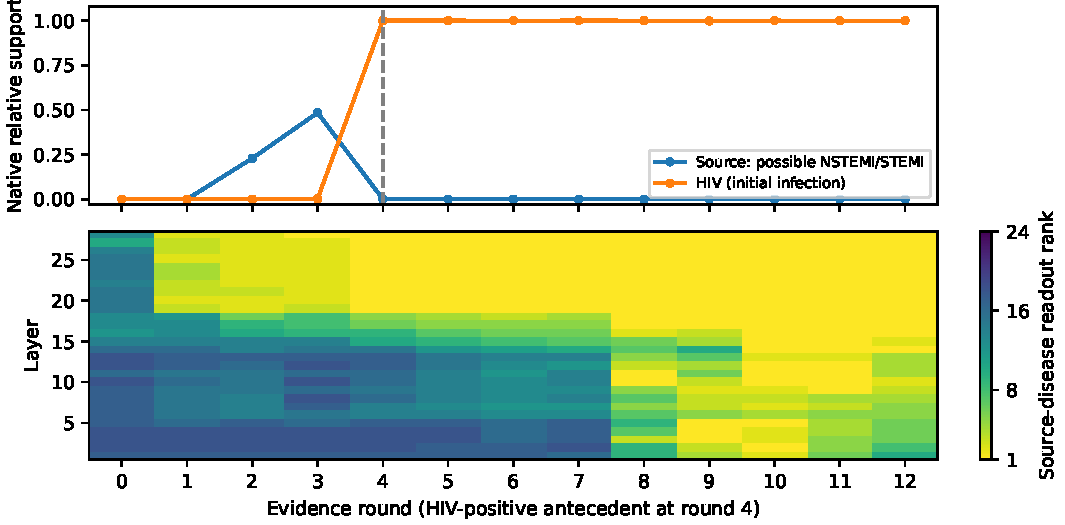
\includegraphics[width=.96\textwidth]{figures/opening_case.pdf}
\caption{Illustrative synthetic patient, selected after observing trajectories. The source diagnosis is possible NSTEMI/STEMI. An HIV-positive antecedent arrives at round 4. Top: native candidate-relative support; bottom: the source disease's rank in independent-patient readouts across all 28 layers. The source record is a 19-year-old female simulation, not an adjudicated or representative clinical case. The example explains the measurement; aggregate results use every preselected trajectory.}\label{fig:opening}
\end{figure*}

\section{Operationalizing Medical Belief}
We do not assign a medical belief to one activation, one attention map, or one confident answer. We measure three properties and their connections.

\paragraph{Content.} Can a state distinguish disease labels for unseen patients? A linear readout trained on separate patients measures decodability. It receives supervision unavailable to native scoring. High probe accuracy alone does not imply task relevance \citep{probing}, and a probe can exploit retained contextual features \citep{contextprobe}. Our simple text and recording-mask controls directly test this concern.

\paragraph{Updating.} Does the disease-related state change when new evidence arrives, and does that change agree with the original model's diagnostic update? We measure continuous disease-pair margins alongside top-class switches. A stable top class may conceal a changing margin; a small margin crossing may change the top class without a large state change.

\paragraph{Influence.} Does changing the observed state component affect the original model's complete disease-name score? The outcome is native output, not the probe score used to define the intervention. We distinguish altering a margin from crossing a decision boundary. These properties provide a computational account of medical belief without assuming subjective experience or a single hidden categorical answer.

\section{Data, Measurements, and Controls}
\paragraph{New patients and independent readouts.}
DDxPlus is a synthetic diagnostic corpus containing patient findings, antecedents, pathology labels, and reference differentials \citep{ddxplus}. We select 240 new official-test patients: ten for each of 24 diseases, grouped into respiratory (60), neurologic (40), cardiovascular (40), digestive (40), ear/nose/throat (30), and systemic (30) cases. Patients are 18--90 years old and have at least five evidence groups. Deterministic selection excludes fact-set duplicates with prior study cohorts, ignoring age and sex. Three patients per disease are preselected for full trajectories. One per disease forms the initial intervention cohort; the remaining two form the independent 48-patient replication cohort.

Layer readouts were fit on an existing, disjoint 120-patient cohort. The new patients are not used to fit weights or choose regularization. For each layer, we normalize the diagnostic-anchor state, subtract the training mean, and apply a ridge readout with fixed regularization 0.1. We use separately trained sequential-input and fixed-questionnaire heads. Their comparison tests decodability under each presentation, not invariance of one shared readout to a layout change.

\paragraph{External cases.}
We select 87 direct diagnosis questions with four original options from the public MedQA test set \citep{medqa}, covering 84 distinct answer strings. Cases must be segmentable and not require external images. We retain original text, split evidence into sentences or intact list blocks, and keep the diagnostic question separate. Reconstructing the input recovers the source text up to whitespace. Selection-rule corrections are archived and precede this module's inference. We do not generate new patient facts or fit the DDxPlus disease readout to these external labels.

\paragraph{What ground truth supports.}
The DDxPlus pathology and MedQA answer are endpoint reference labels. Intermediate prefixes have no adjudicated diagnostic posterior. We therefore describe movement toward, away from, and back to the final source label without calling every early alternative diagnosis an error. DDxPlus pathology equals the maximum reference-differential entry in 171/240 patients; we retain pathology as the main target and report that subset separately.

\paragraph{Models and sequential inputs.}
The primary model is Qwen3-1.7B with 28 layers and FP16 inference; the comparison is Qwen3-4B with 36 layers and 8-bit weights \citep{qwen3}. Both use explicit non-thinking mode. Each natural observation receives cumulative patient facts without earlier model answers. DDxPlus keeps the initial group first and adds subsequent groups in a fixed hash order; this is an evidence-acquisition sequence, not disease progression time. MedQA follows original text order. We record 639 DDxPlus prefixes and 693 MedQA prefixes, giving 1,173 updates across 159 complete trajectories. The second configuration adds 24 paired trajectories. Size and quantization differ together, so it is a configuration replication rather than an isolated scaling experiment.

\paragraph{Native diagnostic scores.}
For a complete candidate string $d$, including its scored termination, we compute
\begin{align}
 L_t(d)&=\sum_j \log p_\theta(d_j\mid x_{\leq t},d_{<j}),\\
 q_t(d)&=\frac{e^{L_t(d)}}{\sum_{c\in\mathcal D}e^{L_t(c)}}.
\end{align}
DDxPlus prompts contain 49 names; the matched readout comparison reranks the same 24 diseases. MedQA uses its four original options. These are candidate-relative string supports, not clinical posterior probabilities. We also store per-token scores, token-mean sensitivity, canonical probability mass, and greedy continuation. This audit matters because surface-form competition can change answer rankings \citep{surface}.

\paragraph{Internal measurements.}
At the final prompt position, every layer contributes five saved arrays: incoming residual, attention increment, post-attention residual, feed-forward increment, and outgoing residual. We also save every query head's anchor attention by input group. Deep natural trajectories include token-level attention, head outputs, and evidence-group endpoint states. Parameter hashes remain unchanged throughout inference; changing activations is not changing model weights.

\paragraph{Statistical unit.}
Endpoints are paired by patient. Dynamic measurements are averaged within patient before summarizing across patients. We report patient-bootstrap 95\% intervals, using an exact binomial boundary interval for all-zero/all-one binary outcomes. Natural intervention tests use 20,000 patient sign permutations and Holm correction over three predetermined layers. The initial and replication cohorts are assessed separately. Appendix~\ref{app:inventory} lists the finite 4,832-condition inventory.

\section{How Diagnoses Form and Change}
Sixty of 72 DDxPlus trajectories change their first-ranked disease at least once; 567 evidence updates yield 170 switches. Fifty-six patients have at least one update changing some candidate support by at least 0.5. MedQA shows 107 switches over 606 updates, with 56/87 vignettes exhibiting a switch and 56/87 a support change of at least 0.5. The large-update criterion is explicitly tied to candidate-relative support.

Paths are heterogeneous (Figure~\ref{fig:paths}). Some retain the source diagnosis, some reach and retain it, some leave and return, and others end elsewhere. Fourteen of 72 DDxPlus patients and 20/87 MedQA vignettes select the source label at some point and later leave it. The largest single step accounts for a patient-mean 43.0\% and 58.8\% of total trajectory variation, respectively. Thus accumulating evidence often produces concentrated turning points rather than a smooth monotonic increase in support for one disease. These are retrospective path descriptions, not six presumed psychological mechanisms.

\begin{figure*}[t]
\centering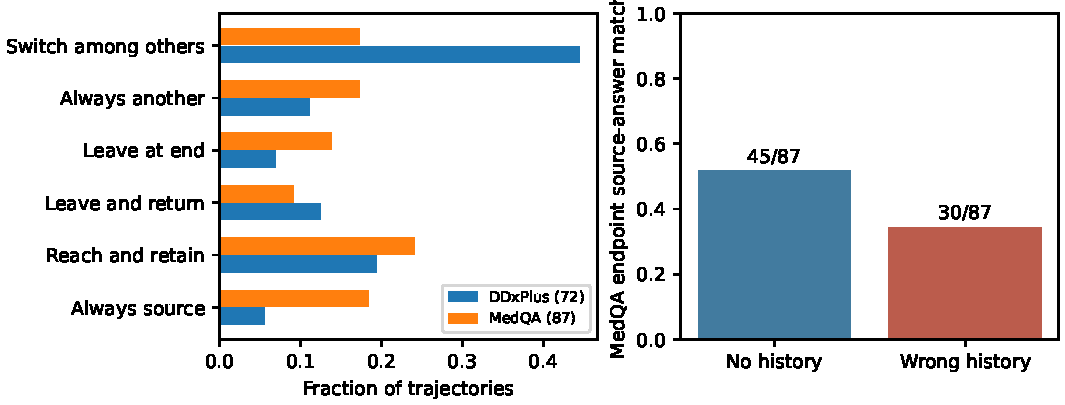
\includegraphics[width=.96\textwidth]{figures/trajectories_history.pdf}
\caption{Left: all preselected trajectories, categorized relative to the complete-case source label. Right: the same 87 complete MedQA vignettes with and without a predetermined wrong prior diagnosis. The paired source-match change is $-17.2$ percentage points (95\% CI $[-27.6,-6.9]$).}\label{fig:paths}
\end{figure*}

\section{Information Availability and Diagnostic Use}
\paragraph{A systematic discrepancy.}
In the matched 24-disease task, native 1.7B scoring identifies 105/240 source labels, while the final-layer readout identifies 194/240, a paired difference of 37.1 percentage points (95\% CI [30.0,44.2]). Both are correct on 93 patients, only the readout on 101, only native scoring on 12, and neither on 34. The discrepancy occurs in all six disease groups (Appendix~\ref{app:groups}), but the readout is not universally correct.

\begin{table}[t]\centering\small
\begin{tabular}{lrrr}\toprule
Configuration & Native 49 & Native 24 & Readout\\\midrule
1.7B sequential & 89/240 & 105/240 & 194/240\\
1.7B panel & 25/240 & 31/240 & 224/240\\
4B sequential & 142/240 & 159/240 & 226/240\\
\bottomrule\end{tabular}
\caption{Source-label matches on the same 240 patients. Native 24 and the readout share the class set. Panel input retains known facts and adds unanswered questionnaire rows.}\label{tab:endpoints}
\end{table}

Fixed-questionnaire presentation makes the discrepancy larger: native 24-disease scoring matches 31/240 labels, whereas the corresponding readout matches 224/240. This preserves known patient facts but changes length and the surrounding unanswered questions. We interpret it as a presentation intervention, not an isolated test of information content or token position.

\paragraph{Interface and data audits.}
Restricting to the 171 cases whose greedy continuation exactly matches a listed canonical name leaves 88 native versus 141 readout matches in the same 24-disease comparison. Restricting to canonical probability mass at least 0.5 leaves 88 versus 143 matches among 173 cases. These output-selected sensitivity subsets do not create independent cohorts, but show that unlisted continuations do not explain the whole difference.

Simple classifiers expose a substantial data shortcut. With the same 120 training patients and unchanged hyperparameters, full-text TF--IDF ridge classification matches 239/240 new labels. Questions without patient answers match 235/240; field presence alone matches 236/240; field/value features match 240/240. Consequently, excellent readout performance is evidence of available source-label information, not sufficient evidence of abstract clinical reasoning. Nor does it establish that a small classifier can replace clinical diagnosis. These controls are part of the explanation, not a separate diagnostic-method claim.

\paragraph{Availability precedes stronger output alignment.}
Layer 14 decodes 162/240 labels, while its patient-mean correlation between internal disease-margin updates and native updates is $-0.040$ (95\% CI $[-0.125,0.048]$). Layer 21 decodes 195/240 with correlation 0.525 [0.421,0.617]; layer 28 decodes 194/240 with correlation 0.573 [0.480,0.660]. Figure~\ref{fig:depth} separates these curves: a state can support disease classification before its changes align strongly with output changes.

For each update, we fix a pair consisting of source disease $g$ and the strongest non-$g$ native competitor $c$ among the 24 classes at the preceding round. We compare
\begin{align}
 \Delta M_t&=\Delta[L_t(g)-L_t(c)],\\
 \Delta S_{t,\ell}&=\Delta[s_{t,\ell}(g)-s_{t,\ell}(c)].
\end{align}
The pair is fixed across the two prefixes of an event. A sensitivity analysis fixing one competitor over the whole trajectory retains final-layer correlation 0.462 [0.351,0.568]. The relationship is therefore not wholly attributable to reselecting competitors.

Among native 24-class switches, the final-layer readout top stays unchanged at a patient-mean rate of 52.7\% [42.3,63.4]. This does not contradict continuous alignment: a margin can move without changing the top class. State movement, disease-margin movement, and top-class movement answer different questions.

\begin{figure*}[t]\centering
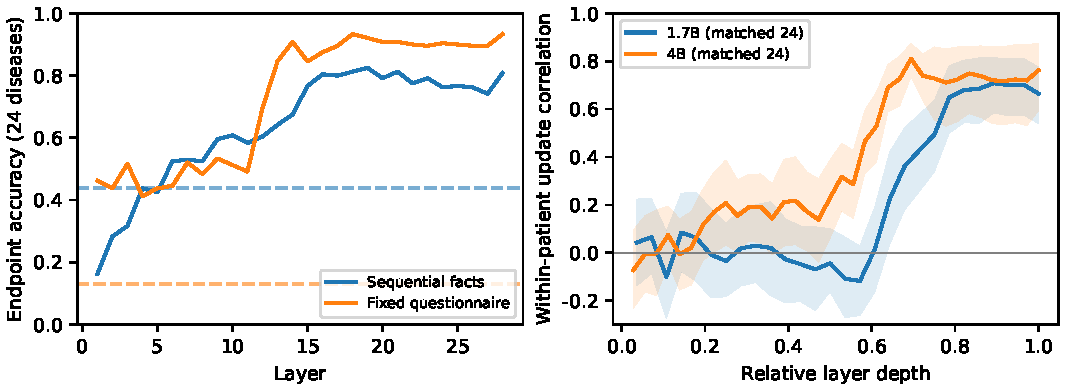
\includegraphics[width=.96\textwidth]{figures/depth.pdf}
\caption{Left: endpoint decodability across depth versus native 24-class scoring (dashed lines), on 240 patients. Right: within-patient association of natural readout and native margin updates, on the same predetermined 24 patients in both configurations. Relative depth accommodates different layer counts. Shading is a patient 95\% interval.}\label{fig:depth}
\end{figure*}

\paragraph{Computational steps.}
Applying the same layer readout to incoming, post-attention, and outgoing normalized states yields an exact telescoping decomposition of its disease-pair margin within that layer. Differencing this decomposition across evidence rounds separates inherited changes from attention-step and feed-forward-step changes. Attention-step differences are pronounced around layer 22 and feed-forward differences at the final layer in the descriptive aggregate. These projections do not identify a unique medical circuit. Their purpose is to locate candidate computational changes for intervention, while the saved token attention describes information access rather than causal importance.

\section{What Conditions Diagnostic Updating?}
\paragraph{Prior diagnoses with current facts held fixed.}
For 24 patients, we insert either the source diagnosis or a predetermined wrong disease as an earlier assistant judgment, with matched message structure and reassessment instruction. The source label is an offline oracle control. We test both a predetermined middle prefix and the full case.
At the middle prefix, correct versus wrong history yields 23/24 versus 1/24 source-label matches. Native top choices change in 22/24 pairs, while the last-layer 24-class readout top changes in 16/24. The two switch rates have different candidate ranges and are reported separately. At the full case, correct versus wrong history yields 23/24 versus 2/24 source-label matches. Native top choices change in 21/24 pairs, while the last-layer 24-class readout top changes in 13/24. The two switch rates have different candidate ranges and are reported separately. The full-case minus middle-prefix change in the matched wrong-versus-source native-margin gain is -0.267 [-6.198, 5.244]; positive values indicate stronger relative historical influence with the additional facts. At the full case, wrong history worsens the source disease's final-layer readout rank by 3.083 [1.417, 5.083] positions on average. Thus the history effect reaches decodable internal information, although the readout may partly encode the inserted disease name rather than a calibrated diagnostic belief. Both histories explicitly state that the preceding assessment may be wrong and request reassessment using only current findings.

The matched experiment compares content of previous judgments; it does not assume that the model truly generated the injected prior. A separate observed-prior condition uses the previous native ranking.

The external MedQA control retains complete current facts and the same reassessment instruction, adding a wrong earlier diagnosis. Source-label matches fall from 45/87 to 30/87. Endorsement of that particular wrong diagnosis increases from 14/87 to 37/87. This external contrast changes the presence of a prior message; the DDxPlus correct/wrong pairing more tightly controls message structure. Together, they show conditions under which existing facts fail to determine a stable answer.

\paragraph{Order, repetition, and evidence context.}
Across 72 DDxPlus patients, reversing subsequent evidence groups changes 30/72 endpoint top choices, and deterministic shuffling changes 20/72. Repeating the middle evidence group changes 5/24 choices in the 24-patient mechanism subset. Repetition adds no new fact, but changes emphasis and position.

In MedQA, reversal changes the selected answer in 23/87 cases and shuffling in 13/87, while both paired accuracy-change intervals contain zero. Stable aggregate accuracy can therefore hide instability in which patients are correctly diagnosed.

We further remove each complete evidence group from 24 full DDxPlus records, giving 208 leave-group-out conditions. For a fixed disease pair, we compare a group's effect when it originally arrived with its effect in the full context. \ContextResult{} Context-dependent sign changes need not be medical reasoning errors; a finding can legitimately support different diagnoses conditional on other evidence. The analysis demonstrates why an evidence update cannot be interpreted as an isolated fixed-weight addition.

\section{Does the Natural Internal Update Matter?}
\paragraph{Removing an observed disease component.}
At a predetermined middle update, let $h_{t,\ell}$ be the new diagnostic-anchor state and $\Delta h_\ell=h_{t,\ell}-h_{t-1,\ell}$. Define a unit disease direction from the independently trained readout:
\begin{equation}
 v_\ell=\frac{W_{\ell,g}-W_{\ell,c}}{\|W_{\ell,g}-W_{\ell,c}\|_2}.
\end{equation}
While retaining the new evidence in the prompt, intervene with
\begin{equation}
 h'_{t,\ell}=h_{t,\ell}-(\Delta h_\ell^\top v_\ell)v_\ell.
\end{equation}
This removes an actually observed update component, rather than choosing an arbitrary positive steering dose. Controls include an equal-norm orthogonal random displacement, zero displacement, and replacement of the entire anchor by its preceding-round value. Layers 14, 21, and 28 are predetermined. The initial cohort contains 24 patients and the independent replication 48; each cohort covers all 24 diseases.

\paragraph{Outcome and replication criterion.}
Let $\delta M$ be the intervention's native-margin effect relative to its zero control. Define attenuation as $A=-\operatorname{sign}(\Delta M)\delta M$. Positive values counteract the original update, irrespective of whether that update favored the source diagnosis. The primary paired contrast is $A_{\rm target}-A_{\rm random}$. We require a positive Holm-significant contrast at the same layer in both cohorts to call the disease-direction effect replicated. We also report top-49 decision changes, because a score effect is weaker than a changed diagnosis.

\begin{table*}[t]\centering\small
\begin{tabular}{lrrrr}\toprule
Layer & First 24: effect [95\% CI] & Holm $p$ & Independent 48: effect [95\% CI] & Holm $p$\\\midrule
14 & 0.009 [-0.008, 0.029] & 0.3632 & -0.008 [-0.021, 0.004] & 0.2546\\
21 & 0.273 [0.041, 0.558] & 0.0578 & 0.262 [0.139, 0.397] & 0.0002\\
28 & 0.645 [0.297, 1.110] & 0.0013 & 0.453 [0.255, 0.702] & 0.0001\\
\bottomrule\end{tabular}
\caption{Removal of natural disease-related update components. Entries are target-minus-random attenuation with patient 95\% intervals; $p$ is Holm-adjusted across three layers separately in each cohort. Native full-name scores are the outcome.}\label{tab:causal}
\end{table*}
Disease-component removal has a replicated, direction-specific native-score effect at layer 28. Table~\ref{tab:causal} reports all three predetermined layers in both cohorts. At layer 28, target removal changes the top-49 diagnosis in 1/24 initial and 1/48 replication patients. Equal-norm random changes do so in 0/24 and 1/48. All zero controls reproduce their corresponding baselines (maximum log-score errors 0.000000 and 0.000000). Score attenuation is therefore evaluated separately from diagnostic boundary crossing.


\paragraph{External natural-state intervention.}
All 87 MedQA vignettes receive a complementary experiment: at the predetermined middle prefix, replace the diagnostic-anchor state by its previous-round value or apply an equal-norm random displacement orthogonal to the natural state difference. No DDxPlus disease probe defines this intervention. \ExternalCausalResult{} This tests the local natural state difference rather than a disease-projection component; the two estimands are not pooled as the same effect.

\begin{figure*}[t]\centering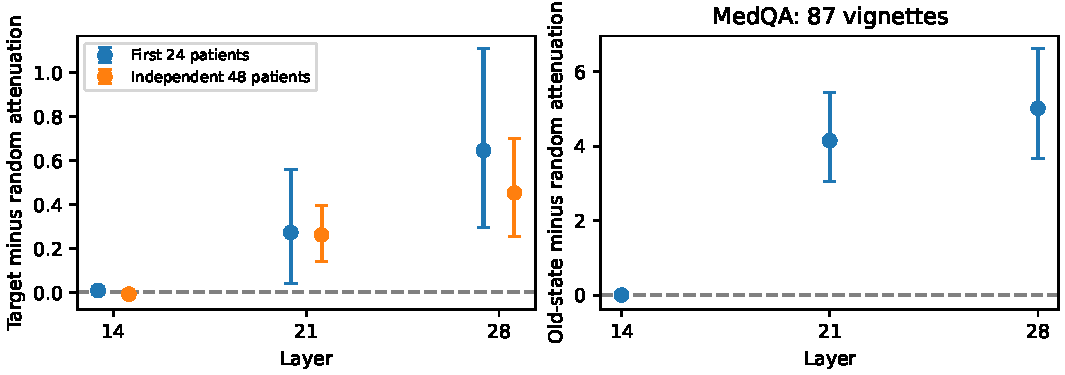
\includegraphics[width=.96\textwidth]{figures/causal.pdf}
\caption{Natural-update interventions with patient 95\% intervals. Left: disease-projection removal in two disjoint DDxPlus cohorts. Right: whole-anchor old-state replacement on MedQA. The intervention definitions differ; both compare native-score attenuation to an equal-norm random control.}\label{fig:causal}
\end{figure*}

\paragraph{Where the causal claim applies.}
Only the final prompt position is changed; other positions and previously computed key/value caches remain intact. At the final layer, a post-feed-forward anchor intervention changes next-token logits but cannot alter later teacher-forced continuation states. Thus, for names sharing the first token, its disease-pair margin effect is exactly zero. We retain this structural negative control. It is a property of the intervention site, not a discovery of a medical module. The supported claim concerns local disease-related changes influencing native name scores, not complete replacement of a model-wide diagnostic belief.

\section{Scope and an Explanatory Follow-up}
\paragraph{Second configuration.}
The 4B configuration identifies 142/240 source labels among 49 diseases, a paired gain of 22.1 points (95\% CI [14.2,30.0]) over 1.7B. In the matched 24-disease comparison, native scoring identifies 159/240 while its final-layer readout identifies 226/240, a gap of 27.9 points (95\% CI [22.1,33.8]). Final-layer natural-update correlation is 0.762 [0.593, 0.876]. The paired 4B-minus-1.7B native switch-rate difference is -0.035 [-0.160, 0.088]; the interval includes zero.

The comparison uses the same 240 endpoints and a predetermined matched 24-patient trajectory subset. Better task performance and elimination of the information--choice discrepancy are different empirical outcomes. Neither the configuration contrast nor layer depth alone establishes that more layers impair medical judgment.

\paragraph{Does explicit fact role resolve the opening case?}
The HIV antecedent in the opening example motivates an exploratory explanation: the model may confuse background history with the current diagnostic target. After observing that case, we test all 72 preselected trajectory patients under three matched role-label conditions: correct source antecedent/current labels, unspecified labels, and swapped labels. The wording of facts, their order, and the role legend are held fixed. Labels derive from source metadata, not the target diagnosis. Swapped labels are counterfactual metadata, not equivalent clinical semantics.
Correct, unspecified, and swapped roles yield 28/72, 31/72, and 29/72 native source-label matches. The paired correct-minus-unspecified change is -4.2 points (95\% CI [-11.1,2.8]). Correct role labeling does not yield a clear aggregate accuracy improvement. Final-layer readout matches in the same three conditions are 54/72, 56/72, and 57/72.

Because the hypothesis was motivated by these patients, this is an explanatory follow-up rather than independent confirmation. Its aggregate result prevents the opening example from becoming an unsupported universal role-confusion mechanism.

\section{Related Work}
\paragraph{Behavioral revision.}
\citet{arun2026} test diagnostic probability coherence on DDxPlus, including order and redundancy; \citet{zeng2026} examine longitudinal clinical judgments and prior assessments. MED-STRESS studies correct judgments under clinical pressure \citep{medstress}, MedEinst builds diagnostic traps \citep{medeinst}, and MedEVM studies evidence value and diagnosis submission \citep{medevm}. DERELAB evaluates defeasible reasoning and confirmation bias in controlled generative tasks \citep{derelab}. These works establish that inconsistency and historical influence are not new observations. Our process-level contribution joins the same natural evidence updates to all-layer information and local interventions.

\paragraph{Internal information and use.}
Medical knowledge maps combine representation analysis, gradients, lesions, and patching \citep{medicalmaps}. Medical contextual/parametric conflict work also distinguishes probe detection from external behavior and uses steering \citep{minpair}. Belief-state geometry has been studied with readouts and interventions in controlled hidden-state tasks \citep{beliefgeometry}. General inference-time interventions \citep{iti} and probe critiques \citep{probing,contextprobe} motivate our separation of decodability, native score influence, and decision changes. We do not claim that medical probing or an information--behavior gap is itself unprecedented. The distinctive evidence here is the connected, same-patient analysis of natural updates, conditional use, and independent-patient component-removal replication.

\section{Discussion and Conclusion}
Medical belief is more usefully investigated as a relationship between available disease information, evidence-induced change, and diagnostic choice than as a single hidden answer. Our measurements expose a depth-dependent relationship: disease information can already be decoded in intermediate layers, while later updates are more closely associated with native diagnostic updates. The same facts can produce different choices under presentation or historical judgments. Local natural-update interventions then test whether these internal changes participate in scoring, separately from whether they can change the chosen diagnosis.

This account accommodates both correct and incorrect readouts, smooth and abrupt trajectories, and successful and unsuccessful explanatory controls. It does not turn a strong classifier on synthetic recording patterns into a clinical breakthrough. Its substantive conclusion is that \emph{information being present, participating in a score, and controlling a choice are empirically distinguishable stages of medical judgment}. The complete trajectory atlas and condition-level records make those stages inspectable across patients rather than only through a compelling anecdote.

\section*{Limitations}
DDxPlus contains strong recording-pattern cues; independent-patient probes can exploit them. External MedQA broadens the evidence source but has only 87 selected diagnostic vignettes and no externally trained disease readout. Neither source supplies ground-truth intermediate posteriors. Native scores depend on canonical answer strings and candidate sets. The two configurations share the Qwen3 family and differ in size and quantization; thinking is disabled. One frozen readout-training cohort does not measure sensitivity to all training samples. Local interventions can leave the natural activation manifold, and the last-layer anchor intervention has first-token selectivity limits. The role-label follow-up is exploratory on observed patients. These boundaries delimit the process analysis rather than being silently replaced by invented clinical validation or global novelty claims.

\section*{Ethics and Reproducibility}
We use pre-existing synthetic records and public exam vignettes, with no collection of private patient data or clinical intervention. Endpoint labels come from the source datasets; we do not invent labels for removed or relabeled evidence. The study is not a validated diagnostic system. Local GPU inference incurs no paid model API usage. Input and source snapshots, model/state hashes, per-token scores, sham checks, and all 4,832 conditions are retained. Manuscript and code development used an AI coding assistant; authors remain responsible for verification and final submission decisions.

\bibliography{references}
\bibliographystyle{acl_natbib}
\clearpage
\appendix
\section{Finite Experimental Inventory}\label{app:inventory}
\begin{table}[H]\centering\small
\begin{tabular}{p{.67\columnwidth}r}\toprule
Module & Conditions\\\midrule
New DDxPlus endpoints, trajectories and primary controls & 1359\\
Initial 24-patient natural component interventions & 288\\
MedQA trajectories and order/history controls & 954\\
4B endpoints and matched trajectories & 424\\
Leave-one-evidence-group-out contexts & 208\\
Matched correct-history full-case supplement & 24\\
Independent 48-patient natural component replication & 576\\
External MedQA natural-state interventions & 783\\
Exploratory source-role labels, 72 patients by three conditions & 216\\\midrule
Total & 4832\\\bottomrule
\end{tabular}
\caption{Configurations and conditions do not add unique patients. There are 240 new DDxPlus patients and 87 MedQA vignettes. All modules are complete.}
\end{table}

\section{Disease Groups and Trajectory Taxonomy}\label{app:groups}
\begin{table}[H]\centering\small
\begin{tabular}{lrrr}\toprule
Group & $N$ & Native 24 & Readout 28\\\midrule
Cardiovascular & 40 & 11 & 27\\
Digestive & 40 & 23 & 36\\
Ent & 30 & 11 & 22\\
Neurologic & 40 & 22 & 35\\
Respiratory & 60 & 32 & 47\\
Systemic & 30 & 6 & 27\\
\bottomrule\end{tabular}
\caption{New-patient endpoint counts by research disease group, 1.7B sequential input.}\end{table}
\begin{table}[H]\centering\small
\begin{tabular}{lrr}\toprule
Trajectory & DDxPlus & MedQA\\\midrule
Always source & 4 & 16\\
Reach and retain & 14 & 21\\
Leave and return & 9 & 8\\
Leave at end & 5 & 12\\
Always another & 8 & 15\\
Switch among others & 32 & 15\\
\bottomrule\end{tabular}
\caption{All 72 DDxPlus and 87 MedQA trajectories. Source refers to the final source label, not a ground-truth intermediate posterior.}\end{table}

\section{Measurement Definitions}
For each complete disease name, we retain token IDs, per-token conditional log probabilities, their sum, candidate-relative support, and probability mass summed over canonical strings. Re-normalizing over the 24-class subset changes the candidate denominator, not the original likelihood of a name. Greedy exact-name accuracy is a string-match diagnostic; an unlisted variant such as ``Acute bronchiolitis'' is not automatically a clinically unrelated answer. We report it separately from likelihood rankings.

Layer readouts apply $s_\ell(h)=W_\ell^\top(h/\|h\|_2-\mu_\ell)+b$. For within-layer decomposition, let $h^{\rm in},h^{\rm att},h^{\rm out}$ denote incoming, post-attention, and outgoing states. For a fixed disease pair, $s(h^{\rm out})=s(h^{\rm in})+[s(h^{\rm att})-s(h^{\rm in})]+[s(h^{\rm out})-s(h^{\rm att})]$, including the appropriate constant cancellation. The same-layer head is applied to all stages. Across-round differences telescope exactly, but do not estimate isolated causal contributions of whole blocks.

Total variation between successive candidate supports is $\frac12\sum_d|q_t(d)-q_{t-1}(d)|$. The largest-step share divides the largest such value by the sum over a trajectory, with zero assigned to a constant path. A ``regression'' means a source-label top choice is followed by a non-source choice; it is a trajectory descriptor, not adjudication of an incomplete clinical prefix. Continuous update correlations require at least three nonconstant paired events. We retain eligible-patient counts with every interval.

For leave-group-out analysis, the competitor is the full-case strongest non-source candidate and remains fixed for both the original arrival effect and the full-context removal effect. Direction comparisons exclude changes smaller than $10^{-4}$ in absolute log margin and include $10^{-3}$ and $10^{-2}$ sensitivity thresholds. Removing an initial group has no preceding natural prefix and is excluded only from the arrival-versus-context sign comparison.

\section{Saved Artifacts and Verification}
Companion files contain Markdown, PNG, and PDF atlases for all 72 DDxPlus, 87 MedQA, and 24 paired configuration trajectories; compressed tables expose candidate and layerwise scores. Raw states and interventions retain patient identifiers. The audit verifies all 4,832 conditions, disjoint facts, input/state/model hashes, probability and attention reconstruction, zero controls, and perturbation norms. GPU code targets MLX/Metal; CUDA requires a matched backend.
\end{document}
